\documentclass{vgtc}

% set font encoding for PDFLaTeX or XeLaTeX
\usepackage{ifxetex}
\ifxetex
  \usepackage{fontspec}
\else
  \usepackage[T1]{fontenc}
  \usepackage[utf8]{inputenc}
  \usepackage{lmodern}
\fi
\usepackage{graphicx}
\usepackage{float}
\usepackage{cite}

% used in maketitle
\title{Study of freight accross Europe.}
\author{Barbier Jeremy, Bazin Adelme, Paffoni Nina}


\begin{document}
\maketitle

\section{Introduction}
In 2015, 323 billions of t-km of goods have been transported in Europe [1]. This freight is highly dominated by the road freight, representing more than 85 percent of the total freight. In this context, it could be interesting to produce visualization about this type of transport. It would be useful for different type of people, from beginners who just want to know a little more about road freight to professional that want to optimize their activities. 
The goal is to highlight the biggest importers or exporters, by type of good or in general, and the countries between which there is the more exchange. For a professional use of these visualization, it could help the user to know which country to target if he wants to transport such-and-such type of good.

# Détailler avec l'utilisation qu'en ferait un utilisateur lambda (par exemple info sur l'importe export de catégorie comme le pétrole, le tabac...
# Permet d'avoir une visualisation globale, ce qui n'est pas le cas là ou on a pris les données (eurostat)


Another purpose of the map is the link made with the time. Data are shown by year, which allows the user to make a link with events like political change, or climate disaster. 


\section{Related Work}

\begin{figure}[H]
\center
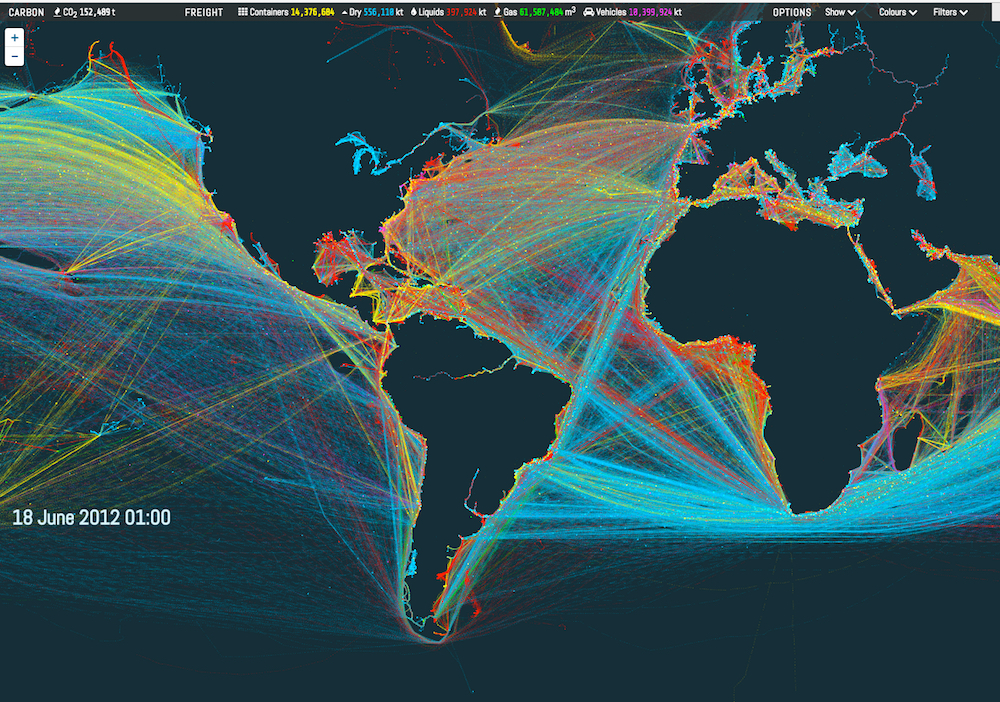
\includegraphics[scale=0.2]{shipmap.jpg}
\end{figure}

\begin{figure}[H]
\center
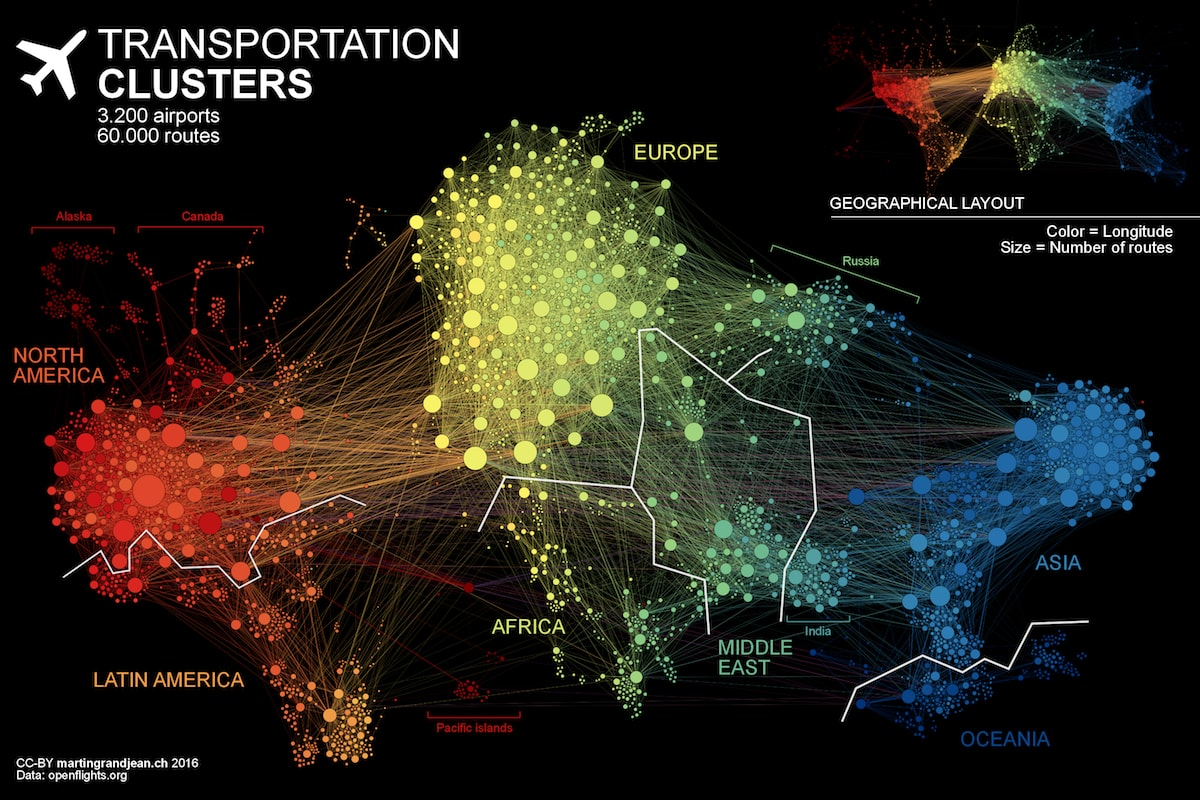
\includegraphics[scale=0.15]{airports-network-small.jpg}
\end{figure}

\begin{figure}[H]
\center
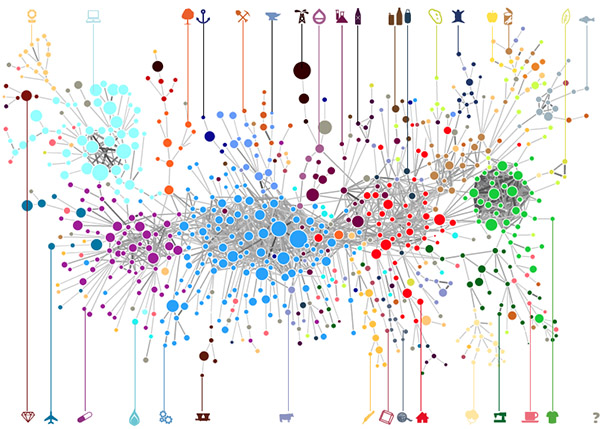
\includegraphics[scale=0.4]{economic_growth_atlas2.jpg}
\end{figure}

# Dire où on a pris les données, et qu'il y a pas de visu globale vis à vis de celles ci
# Ajouter une gridmap (OD map)

\section{Project Description}
# Description des données, et comment on les a modifié (csvTojson) pour les rendre utilisables avec js 
# Intérêt de la représentation en gridmap

\subsection{Grid map}
A tile grid map or simple grid map is a representation of a geographic area divided into a set of equal squares\cite{Good Data Visualization Practice: Tile Grid Maps}.
The grid map is an unconventionnal choice to represent a geographic area but presents interesting advantages in our context. One of them is that supress the information of the superficie of the country which is not relevant in this case and which can be a visual biais that lead the user to accord more importance to largest countries. Furthermore, by simply represent each country by a squarre allow us to developp small multiple visualization (OD maps). You can notice that we add a toogle button that allow the user to change with an animation the grid map to the classic map with mercator projection. This permit for the user to easily understand what this grid map represent and which squarre reppresent each country. 

%on pourrait mettre 2 images : une de notre carte sous forme chloroplete et une de notre carte sous forme gridmap (mais sans les OD maps)
%keywords : #distortion #chloropleth 

\subsection{OD maps}
# Formes simples (carré), donc visuellement plus facile à appréhender que si on avait des formes plus différentes (carte classique)
# De plus, permet d'intégrer la map dans chaque carré, ce qui ne serait pas possible avec une carte normale. OD map (grid map dans une grid map) permet d'avoir des motifs dans chaque pays, et donc facilite la comparaison entre 2 pays. Faisable car sur l'Europe, une trentaine de pays, car si sur le monde entier trop d'informations. 
# Le seul inconvénient, c'est que le fait que ce soit l'Europe saute pas aux yeux, c'est pour ça qu'on a conservé la carte classique de base, et qu'on a ajouté un tooltip  
# Choix d'intensité de couleurs pour visualiser l'intensité du traffic, car c'est simple à comprendre. Pays par pays (avec le max du pays), car sinon on risquait d'avoir une concentration sur les plus gros consommateur/producteurs (France/Allemagne/Angleterre)
# Pour naviguer, choix de checkbox car c'est le plus facile d'utilisation pour l'utilisateur
# Même justification pour la scrollbar des années 

\begin{figure}[H]
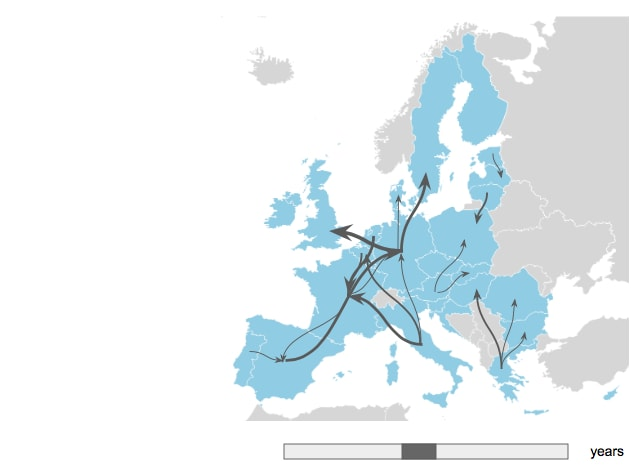
\includegraphics[scale=0.35]{Capture_ecran_2017-11-29_171310.jpg}
\caption{Proposition of global visualization, showing flow of freight across UE}
\end{figure}

\begin{figure}[H]
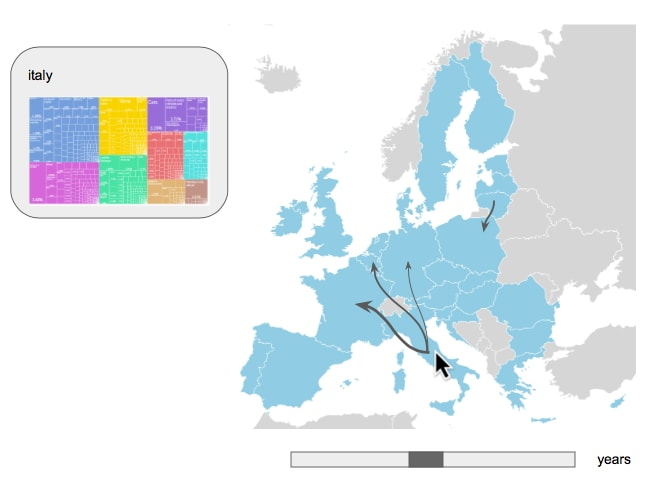
\includegraphics[scale=0.35]{Capture_ecran_2017-11-29_171255.jpg}
\caption{By clicking on a specific country (here Italy), the user will see only the flow of goods that involve the country and display details concerning types of goods}
\end{figure}


\section{Discussion}
# Bien : simplicité de la visualisation par rapport à la complexité des données. Il faut comprendre ici que sur la carte sont représentées tous les échanges entre pays européens sur une année, donc quelque chose d'extrêmement complexe, et que ça reste malgré tout lisible et compréhensible, et qu'il est assez facile de voir entre quels pays il y a beaucoup d'échange, ou s'il y a une tendance (nord-sud/est-ouest par exemple).
# Intérêt : Par exemple, on voit que lorsque on regarde de manière globale, on a assez peu de changement dans le temps dans la quantité d'échange entre les pays. Par contre si on regarde de manière plus détaillée, on a beaucoup plus de différence. Ce qui laisse l'utilisateur très libre quand à ce qu'il veut analyser.
# Choix de couleur par pays, du coup on le justifie dans la discussion, mais ça empeche d'avoir une comparaison brute entre les pays directement (en terme de t-km par exemple)
# Ouverture : Jeu de données plus détaillé serait intéressant (exemple on voit des différences pour l'agriculture mais on peut pas dire que ça vient de tel ou tel produit)

\section{Conclusion \& Perspectives}
# Il y avait pas de visu sur les transports routiers, ou en tout cas pas sur eurostat. Suffisamment simple pour être comprise rapidement. Et si on s'y attarde, on peut y trouver énormément de données différentes et faire beaucoup d'analyses.


\bibliographystyle{plain}
\bibliography{template}
\end{document}
